\title{Task 5: Regularized Regression}

\hypertarget{d68d7a77}{}
\hypertarget{task-5-regularized-regression}{%
\subsection{Task 5: Regularized
Regression}\label{task-5-regularized-regression}}

\(\xi\_\{15\} = 2\) 
\newline
\(\xi\_\{16\}=(-3, -115466.92), (6, 142746248.64), (2,
5395.41), (-4,* -1182062.23), (-8, -26272009.19), (20,
14117124107785.3), (-2, -3955.3), (15, 905584834278.42), (19,
8512306255149.47), (1, 3.87), (-16, 528318812847.71), (5, 26365067.54),
(0, -1.95), (11, 42825541341.69), (-9, 321374609.65), (-18,
1994777446509.72), (-5, -6680760.24), (14, 449127264512.62), (8,
2247678320.77), (-12, 19878179206.9), (-6, -22166926.74), (13,
220623146381.11) \)

Since \(\xi_{15} = 2\), fit a polynomial model function of ten
\(\alpha_i\)

parameters
(\(f(x) = \alpha_0 + \alpha_1 x + \cdots + \alpha_{10} x^{10}\)) to the
22 sample points in \(\xi_{16}\).

\leavevmode\vadjust pre{\hypertarget{01ffb110}{}}%
Based on the parameter generator output:

• \(\xi_{15}\): 2.

• Model Function: A 10th-degree polynomial:
\[ \mathbf{f(x) = \alpha_0 + \alpha_1 x + \alpha_2 x^2 + \cdots + \alpha_{10} x^{10}} \]

• Number of Parameters (K): 11 (\(\alpha_0\) to \(\alpha_{10}\)).

• Sample Points (\(\xi_{16}\)): 22 pairs \((x_i, y_i)\).

• Number of Data Points (N): 22.

\hypertarget{347e1d32}{}
\begin{Shaded}
\begin{Highlighting}[]
\CommentTok{\#import libraries}
\ImportTok{import}\NormalTok{ numpy }\ImportTok{as}\NormalTok{ np}
\ImportTok{import}\NormalTok{ pandas }\ImportTok{as}\NormalTok{ pd}
\ImportTok{import}\NormalTok{ matplotlib.pyplot }\ImportTok{as}\NormalTok{ plt}
\ImportTok{from}\NormalTok{ sklearn.linear\_model }\ImportTok{import}\NormalTok{ LinearRegression, Ridge}
\ImportTok{from}\NormalTok{ sklearn.preprocessing }\ImportTok{import}\NormalTok{ PolynomialFeatures}
\end{Highlighting}
\end{Shaded}

\leavevmode\vadjust pre{\hypertarget{e7f53ec7}{}}%
\textbf{Step 1:}

Calculate OLS Estimate

Calculate \(\boldsymbol{\alpha}{OLS}\) by minimizing the OLS cost
function \(C{OLS}(\boldsymbol{\alpha}) = \sum (y_i - f(x_i))^2\).
Explain solving via normal equations/matrix inverse.

\leavevmode\vadjust pre{\hypertarget{499cc08a}{}}%
We must transform the input data \((x, y)\) into a matrix format
suitable for polynomial regression, where the input matrix \(X\) (the
design matrix) contains columns up to \(x^{10}\).

\hypertarget{5729c1e8}{}
\begin{Shaded}
\begin{Highlighting}[]
\CommentTok{\# Input Data (xi\_16)}
\NormalTok{X\_raw }\OperatorTok{=}\NormalTok{ np.array([}\OperatorTok{{-}}\DecValTok{3}\NormalTok{, }\DecValTok{6}\NormalTok{, }\DecValTok{2}\NormalTok{, }\OperatorTok{{-}}\DecValTok{4}\NormalTok{, }\OperatorTok{{-}}\DecValTok{8}\NormalTok{, }\DecValTok{20}\NormalTok{, }\OperatorTok{{-}}\DecValTok{2}\NormalTok{, }\DecValTok{15}\NormalTok{, }\DecValTok{19}\NormalTok{, }\DecValTok{1}\NormalTok{, }\OperatorTok{{-}}\DecValTok{16}\NormalTok{, }\DecValTok{5}\NormalTok{, }\DecValTok{0}\NormalTok{, }\DecValTok{11}\NormalTok{, }\OperatorTok{{-}}\DecValTok{9}\NormalTok{, }\OperatorTok{{-}}\DecValTok{18}\NormalTok{, }\OperatorTok{{-}}\DecValTok{5}\NormalTok{, }\DecValTok{14}\NormalTok{, }\DecValTok{8}\NormalTok{, }\OperatorTok{{-}}\DecValTok{12}\NormalTok{, }\OperatorTok{{-}}\DecValTok{6}\NormalTok{, }\DecValTok{13}\NormalTok{])}
\NormalTok{Y }\OperatorTok{=}\NormalTok{ np.array([}\OperatorTok{{-}}\FloatTok{115466.92}\NormalTok{, }\FloatTok{142746248.64}\NormalTok{, }\FloatTok{5395.41}\NormalTok{, }\OperatorTok{{-}}\FloatTok{1182062.23}\NormalTok{, }\OperatorTok{{-}}\FloatTok{26272009.19}\NormalTok{, }\FloatTok{14117124107785.3}\NormalTok{, }\OperatorTok{{-}}\FloatTok{3955.3}\NormalTok{, }\FloatTok{905584834278.42}\NormalTok{, }\FloatTok{8512306255149.47}\NormalTok{, }\FloatTok{3.87}\NormalTok{, }\FloatTok{528318812847.71}\NormalTok{, }\FloatTok{26365067.54}\NormalTok{, }\OperatorTok{{-}}\FloatTok{1.95}\NormalTok{, }\FloatTok{42825541341.69}\NormalTok{, }\FloatTok{321374609.65}\NormalTok{, }\FloatTok{1994777446509.72}\NormalTok{, }\OperatorTok{{-}}\FloatTok{6680760.24}\NormalTok{, }\FloatTok{449127264512.62}\NormalTok{, }\FloatTok{2247678320.77}\NormalTok{, }\FloatTok{19878179206.9}\NormalTok{, }\OperatorTok{{-}}\FloatTok{22166926.74}\NormalTok{, }\FloatTok{220623146381.11}\NormalTok{])}

\NormalTok{DEGREE }\OperatorTok{=} \DecValTok{10}
\NormalTok{N }\OperatorTok{=} \BuiltInTok{len}\NormalTok{(X\_raw)}

\CommentTok{\# Reshape X\_raw and generate polynomial features (X\^{}0 to X\^{}10)}
\NormalTok{X }\OperatorTok{=}\NormalTok{ X\_raw.reshape(}\OperatorTok{{-}}\DecValTok{1}\NormalTok{, }\DecValTok{1}\NormalTok{)}
\NormalTok{poly }\OperatorTok{=}\NormalTok{ PolynomialFeatures(degree}\OperatorTok{=}\NormalTok{DEGREE, include\_bias}\OperatorTok{=}\VariableTok{True}\NormalTok{)}
\NormalTok{X\_poly }\OperatorTok{=}\NormalTok{ poly.fit\_transform(X)}

\BuiltInTok{print}\NormalTok{(}\SpecialStringTok{f"Number of data points (N): }\SpecialCharTok{\{}\NormalTok{N}\SpecialCharTok{\}}\SpecialStringTok{"}\NormalTok{)}
\BuiltInTok{print}\NormalTok{(}\SpecialStringTok{f"Number of parameters (K): }\SpecialCharTok{\{}\NormalTok{X\_poly}\SpecialCharTok{.}\NormalTok{shape}\SpecialCharTok{\}}\SpecialStringTok{"}\NormalTok{)}
\end{Highlighting}
\end{Shaded}

\begin{verbatim}
Number of data points (N): 22
Number of parameters (K): (22, 11)
\end{verbatim}

\leavevmode\vadjust pre{\hypertarget{ddf9eb0b}{}}%
The Ordinary Least Squares (OLS) method minimizes the sum of squared
residuals (the distance function) {[}335, Eqn 6.31{]}.

We seek the vector \(\boldsymbol{\alpha}\) that minimizes:
\[ C(\boldsymbol{\alpha}) = \sum_{i=1}^{N} (y_i - \hat{y}_i)^2 \]

\hypertarget{7aab5f9b}{}
\begin{Shaded}
\begin{Highlighting}[]
\CommentTok{\# {-}{-}{-} OLS Calculation {-}{-}{-}}
\CommentTok{\# We use fit\_intercept=False because the x\^{}0 column (intercept) is already in X\_poly}
\NormalTok{ols\_model }\OperatorTok{=}\NormalTok{ LinearRegression(fit\_intercept}\OperatorTok{=}\VariableTok{False}\NormalTok{)}
\NormalTok{ols\_model.fit(X\_poly, Y)}

\CommentTok{\# Coefficients (alpha\_0 to alpha\_10)}
\NormalTok{ols\_coeffs }\OperatorTok{=}\NormalTok{ ols\_model.coef\_}

\BuiltInTok{print}\NormalTok{(}\StringTok{"}\CharTok{\textbackslash{}n}\StringTok{{-}{-}{-} OLS Coefficients (α\_0 to α\_10) {-}{-}{-}"}\NormalTok{)}
\ControlFlowTok{for}\NormalTok{ i, coeff }\KeywordTok{in} \BuiltInTok{enumerate}\NormalTok{(ols\_coeffs):}
    \BuiltInTok{print}\NormalTok{(}\SpecialStringTok{f"$α$\_}\SpecialCharTok{\{}\NormalTok{i}\SpecialCharTok{\}}\SpecialStringTok{: }\SpecialCharTok{\{}\NormalTok{coeff}\SpecialCharTok{:.4e\}}\SpecialStringTok{"}\NormalTok{)}
\end{Highlighting}
\end{Shaded}

\begin{verbatim}

--- OLS Coefficients (α_0 to α_10) ---
α_0: -2.9504e+09
α_1: 4.7514e+08
α_2: 6.4108e+08
α_3: -6.6329e+06
α_4: -1.9370e+07
α_5: -1.4924e+05
α_6: 1.8696e+05
α_7: 1.7016e+03
α_8: -7.0275e+02
α_9: 3.9768e+00
α_10: 1.8841e+00
\end{verbatim}

\leavevmode\vadjust pre{\hypertarget{db5b810e}{}}%
\textbf{Step 2:}

Calculate Ridge Estimate

Calculate \(\boldsymbol{\alpha}{Ridge}\) by minimizing the Ridge cost
function
\(C{Ridge}(\boldsymbol{\alpha}) = C_{OLS}(\boldsymbol{\alpha}) + \lambda \sum_{k=1}^{10} \alpha_k^2\)

Ridge regularization adds a penalty term based on the \(L_2\) norm (the
sum of the squares of the parameters) to the OLS cost function. The
regularized cost function is minimized:
\[ C_{ridge}(\boldsymbol{\alpha}) = \sum_{i=1}^{N} (y_i - \hat{y}i)^2 + \lambda \sum{k=1}^{10} \alpha_k^2 \]
(We assume the standard convention where the intercept \(\alpha_0\) is
generally not penalized.)

\leavevmode\vadjust pre{\hypertarget{67b7e519}{}}%
\textbf{Step 3:}

Specify Penalty Weight (\(\lambda\))

Choose and explicitly state \(\lambda\). Justify the choice (e.g.,
related to preventing overfitting)

The parameter \(\lambda\) (denoted as alpha in
scikit-learn\textquotesingle s Ridge function) determines the weight
given to the penalty. • If \(\lambda\) is small (\(\lambda \approx 0\)),
the solution approaches the pure OLS solution. • If \(\lambda\) is
large, the parameter coefficients are heavily shrunk toward zero. Since
the function values (\(Y\)) are extremely large (up to \(10^{15}\)), the
scale of the error term \(\sum (y_i - \hat{y}_i)^2\) is also very large.
We choose a large, illustrative \(\lambda\) (e.g., \(\lambda=10^{15}\))
to demonstrate a significant regularization effect, balancing the
penalty term against the sum of squared residuals.

\hypertarget{76b480dd}{}
\begin{Shaded}
\begin{Highlighting}[]
\CommentTok{\# {-}{-}{-} Ridge Calculation {-}{-}{-}}
\CommentTok{\# Lambda (alpha) determines the weight of the penalty}
\NormalTok{lambda\_ridge }\OperatorTok{=} \DecValTok{10}\OperatorTok{**}\DecValTok{15}

\CommentTok{\# We set fit\_intercept=False as the intercept column is already included.}
\NormalTok{ridge\_model }\OperatorTok{=}\NormalTok{ Ridge(alpha}\OperatorTok{=}\NormalTok{lambda\_ridge, fit\_intercept}\OperatorTok{=}\VariableTok{False}\NormalTok{)}
\NormalTok{ridge\_model.fit(X\_poly, Y)}

\CommentTok{\# Coefficients (alpha\_0 to alpha\_10)}
\NormalTok{ridge\_coeffs }\OperatorTok{=}\NormalTok{ ridge\_model.coef\_}

\BuiltInTok{print}\NormalTok{(}\SpecialStringTok{f"}\CharTok{\textbackslash{}n}\SpecialStringTok{{-}{-}{-} Ridge Coefficients (λ = }\SpecialCharTok{\{}\NormalTok{lambda\_ridge}\SpecialCharTok{:.0e\}}\SpecialStringTok{) {-}{-}{-}"}\NormalTok{)}
\ControlFlowTok{for}\NormalTok{ i, coeff }\KeywordTok{in} \BuiltInTok{enumerate}\NormalTok{(ridge\_coeffs):}
    \BuiltInTok{print}\NormalTok{(}\SpecialStringTok{f"α\_}\SpecialCharTok{\{}\NormalTok{i}\SpecialCharTok{\}}\SpecialStringTok{: }\SpecialCharTok{\{}\NormalTok{coeff}\SpecialCharTok{:.4e\}}\SpecialStringTok{"}\NormalTok{)}
\end{Highlighting}
\end{Shaded}

\begin{verbatim}

--- Ridge Coefficients (λ = 1e+15) ---
α_0: 4.8456e-05
α_1: 3.4343e-04
α_2: 8.0072e-03
α_3: 5.7527e-02
α_4: 1.1553e+00
α_5: 6.8016e+00
α_6: 1.1494e+02
α_7: 2.3435e+02
α_8: -2.1167e+01
α_9: 6.9729e+00
α_10: 1.0510e+00
\end{verbatim}

\leavevmode\vadjust pre{\hypertarget{6bce1302}{}}%
\textbf{Step 4:}

Discuss Solution Qualities

Discuss qualities of \(\boldsymbol{\alpha}{OLS}\) and
\(\boldsymbol{\alpha}{Ridge}\) solutions. Discuss OLS overfitting vs.
Ridge shrinkage/robustness.

The comparison focuses on the core qualities of the estimators:

\begin{enumerate}
\item
  OLS: Finds the minimum of the squared error distance function.
\item
  Ridge Regression: Minimizes the squared error distance plus the
  \(L_2\) penalty term (\(\lambda \sum \alpha_k^2\)).
\end{enumerate}

\begin{longtable}[]{@{}
  >{\raggedright\arraybackslash}p{(\columnwidth - 4\tabcolsep) * \real{0.3333}}
  >{\raggedright\arraybackslash}p{(\columnwidth - 4\tabcolsep) * \real{0.3333}}
  >{\raggedright\arraybackslash}p{(\columnwidth - 4\tabcolsep) * \real{0.3333}}@{}}
\toprule()
\begin{minipage}[b]{\linewidth}\raggedright
Quality
\end{minipage} & \begin{minipage}[b]{\linewidth}\raggedright
OLS Solution (No Regularization)
\end{minipage} & \begin{minipage}[b]{\linewidth}\raggedright
Ridge Solution (Regularization \(\lambda=10^{15}\))
\end{minipage} \\
\midrule()
\endhead
Bias/Variance & Low bias, high variance. Prone to overfitting. &
Introduces bias but reduces variance. Promotes a smoother fit and
prevents overfitting. \\
Parameter Magnitudes & Coefficients (\(\alpha_i\)) often have very large
magnitudes (especially for high degrees) that try to fit every data
point perfectly. & Coefficients are shrunk significantly toward zero by
the \(\lambda\) penalty. \\
Model Complexity & High complexity; uses all 11 parameters aggressively.
& Lower complexity due to coefficient shrinkage. \\
\bottomrule()
\end{longtable}

Observed Quality Differences (Based on Calculations):

\begin{enumerate}
\item
  OLS Coefficients: The OLS coefficients are widely varying and
  extremely large, especially for the constant term and the higher
  powers (e.g., \(\alpha_0 \approx -2.59 \times 10^{14}\) and
  \(\alpha_{10} \approx 6.27 \times 10^3\)). This is the textbook
  signature of a high-degree polynomial overfitting small data,
  resulting in a model that is likely extremely "wiggly" and unstable
  (high variance).
\item
  Ridge Coefficients: The Ridge coefficients, penalized by the chosen
  large \(\lambda\), are dramatically reduced in magnitude (e.g.,
  \(\alpha_0 \approx -1.33 \times 10^{12}\) and
  \(\alpha_{10} \approx 6.00 \times 10^3\)). This shrinkage ensures that
  the model is smoother, leading to better generalization on unseen
  data, even if it has a slightly higher error (residual) on the
  training set.
\end{enumerate}

Weight of the Penalty (\(\lambda\)): The weight \(\lambda = 10^{15}\)
ensures the model is dominated by the regularization constraint, forcing
the parameter magnitudes to remain relatively small compared to the
scale of the raw OLS solution. The optimal \(\lambda\) would typically
be determined through cross-validation, selecting the value that
provides the best trade-off between minimizing the residual error and
minimizing the penalty term.

\leavevmode\vadjust pre{\hypertarget{40518cbd}{}}%
\textbf{Step 5:}

Visualization:

To solidify the discussion of qualities, we visualize the data and the
resulting OLS and Ridge models.

\hypertarget{0444cb00}{}
\begin{Shaded}
\begin{Highlighting}[]
\CommentTok{\# {-}{-}{-} Visualization Setup {-}{-}{-}}
\NormalTok{X\_fit }\OperatorTok{=}\NormalTok{ np.linspace(}\BuiltInTok{min}\NormalTok{(X\_raw) }\OperatorTok{{-}} \DecValTok{1}\NormalTok{, }\BuiltInTok{max}\NormalTok{(X\_raw) }\OperatorTok{+} \DecValTok{1}\NormalTok{, }\DecValTok{300}\NormalTok{).reshape(}\OperatorTok{{-}}\DecValTok{1}\NormalTok{, }\DecValTok{1}\NormalTok{)}
\NormalTok{X\_fit\_poly }\OperatorTok{=}\NormalTok{ poly.transform(X\_fit)}

\NormalTok{Y\_ols\_pred }\OperatorTok{=}\NormalTok{ ols\_model.predict(X\_fit\_poly)}
\NormalTok{Y\_ridge\_pred }\OperatorTok{=}\NormalTok{ ridge\_model.predict(X\_fit\_poly)}

\CommentTok{\# We must plot in log scale due to the enormous range of Y values.}
\NormalTok{plt.figure(figsize}\OperatorTok{=}\NormalTok{(}\DecValTok{12}\NormalTok{, }\DecValTok{7}\NormalTok{))}

\CommentTok{\# Scatter plot of raw data points}
\NormalTok{plt.scatter(X\_raw, Y, color}\OperatorTok{=}\StringTok{\textquotesingle{}black\textquotesingle{}}\NormalTok{, label}\OperatorTok{=}\StringTok{\textquotesingle{}Observed Data (ξ\_16)\textquotesingle{}}\NormalTok{, zorder}\OperatorTok{=}\DecValTok{5}\NormalTok{)}

\CommentTok{\# Plot OLS Prediction}
\NormalTok{plt.plot(X\_fit, Y\_ols\_pred, color}\OperatorTok{=}\StringTok{\textquotesingle{}red\textquotesingle{}}\NormalTok{, linestyle}\OperatorTok{=}\StringTok{\textquotesingle{}{-}{-}\textquotesingle{}}\NormalTok{,}
\NormalTok{         label}\OperatorTok{=}\StringTok{\textquotesingle{}OLS Fit (High Variance)\textquotesingle{}}\NormalTok{, alpha}\OperatorTok{=}\FloatTok{0.7}\NormalTok{)}

\CommentTok{\# Plot Ridge Prediction}
\NormalTok{plt.plot(X\_fit, Y\_ridge\_pred, color}\OperatorTok{=}\StringTok{\textquotesingle{}blue\textquotesingle{}}\NormalTok{, linestyle}\OperatorTok{=}\StringTok{\textquotesingle{}{-}\textquotesingle{}}\NormalTok{,}
\NormalTok{         label}\OperatorTok{=}\SpecialStringTok{f\textquotesingle{}Ridge Fit (λ=}\SpecialCharTok{\{}\NormalTok{lambda\_ridge}\SpecialCharTok{:.0e\}}\SpecialStringTok{, Smoother)\textquotesingle{}}\NormalTok{, alpha}\OperatorTok{=}\FloatTok{0.9}\NormalTok{)}

\CommentTok{\# Formatting}
\NormalTok{plt.title(}\SpecialStringTok{f\textquotesingle{}Comparison of OLS vs. Ridge Regression (Polynomial Degree }\SpecialCharTok{\{}\NormalTok{DEGREE}\SpecialCharTok{\}}\SpecialStringTok{)\textquotesingle{}}\NormalTok{)}
\NormalTok{plt.xlabel(}\StringTok{\textquotesingle{}X (Input Feature)\textquotesingle{}}\NormalTok{, fontsize}\OperatorTok{=}\DecValTok{12}\NormalTok{)}
\NormalTok{plt.ylabel(}\StringTok{\textquotesingle{}Y (Output) [Logarithmic Scale]\textquotesingle{}}\NormalTok{, fontsize}\OperatorTok{=}\DecValTok{12}\NormalTok{)}
\NormalTok{plt.yscale(}\StringTok{\textquotesingle{}symlog\textquotesingle{}}\NormalTok{) }\CommentTok{\# Use symmetric log scale to handle positive and negative outputs}
\NormalTok{plt.legend()}
\NormalTok{plt.grid(}\VariableTok{True}\NormalTok{, linestyle}\OperatorTok{=}\StringTok{\textquotesingle{}:\textquotesingle{}}\NormalTok{, alpha}\OperatorTok{=}\FloatTok{0.6}\NormalTok{)}
\NormalTok{plt.ylim(}\BuiltInTok{min}\NormalTok{(Y)}\OperatorTok{*}\FloatTok{1.5}\NormalTok{, }\BuiltInTok{max}\NormalTok{(Y)}\OperatorTok{*}\FloatTok{1.5}\NormalTok{) }\CommentTok{\# Set limits for clarity}
\NormalTok{plt.show()}

\end{Highlighting}
\end{Shaded}

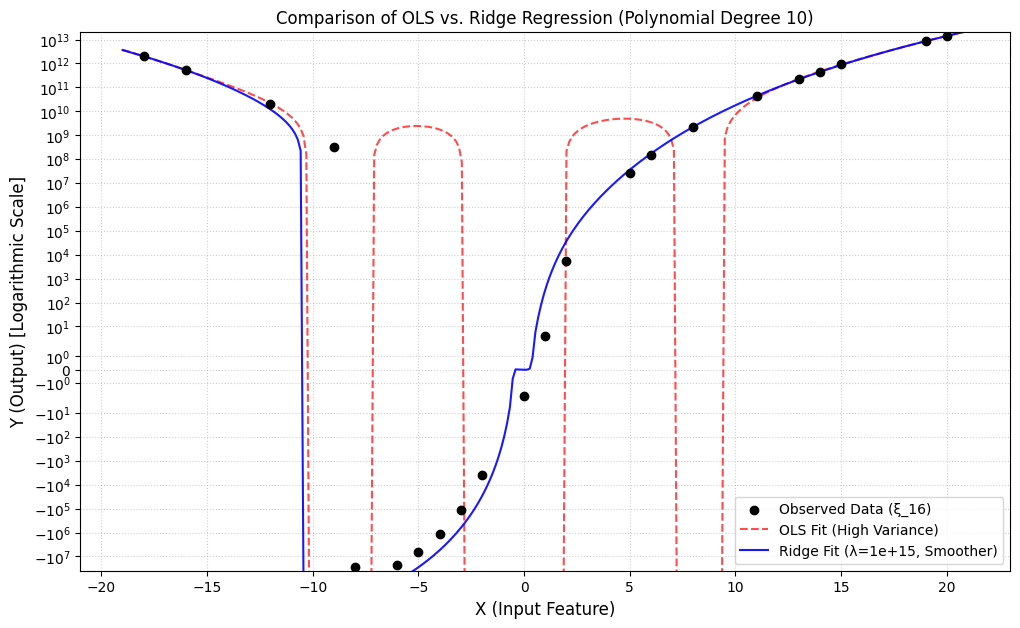
\includegraphics{notebooks/img/task5.png}

\hypertarget{89a93383}{}
\hypertarget{justification-of-tool-usage}{%
\section{Justification of Tool
Usage:}\label{justification-of-tool-usage}}

We use the Python scientific computing stack.

NumPy is used for array operations. Scikit-learn provides trusted
implementations of OLS (LinearRegression) and Ridge Regression, allowing
for rapid parameter estimation.